\documentclass[onecolumn]{article}
\usepackage{CJKutf8, graphicx}%导入CJKutf8包,并且激活中文、日文、韩文的uft8编码
\usepackage[utf8]{inputenc}
\usepackage{setspace}
\usepackage{indentfirst}
\usepackage{geometry}
\geometry{left=3.18cm,right=3.18cm,top=2.54cm,bottom=2.54cm}
\renewcommand{\baselinestretch}{1.5}

\title{短视频传输实验报告}
\author{计研173 \quad 陈雨兰 \quad 2017310787  \\ 计研173 \quad 蔡文静 \quad 2017210866}
\date{January 2018}

\begin{document}
	\begin{CJK*}{UTF8}{gbsn}
		
		\maketitle
\section{介绍}
		本实验项目实现了从客户端到服务器端的短视频快速上传。我们在UDP协议传输数据的基础上加上了乱序恢复、丢包恢复和请求重传,从而实现了短视频的快速准确的传输。
		
\section{项目设计与分析}
		\subsection{算法框架}
		为了应对UDP传输中的丢包和乱序的情况,我们采用前向纠错技术进行丢包恢复。
		该算法由发送方进行FEC编码引入冗余包,接收方进行FEC解码并恢复丢失的数据包。
		对于包乱序和包重复,我们采用QOS乱序恢复处理。
		%该QOS方案特点是在没有丢包的情况下,不引入任何系统延时,并且可以通过可控的丢包等待时延来适应不同的信道乱序程度。
		QOS需要在接收端进行FEC解码前进行,确保送FEC解码模块的数据包序号是正确的(不存在乱序,仅存在丢包)。
		图\ref{fig:frame}为算法的主要框架。
		
		\begin{figure}[h]
			\centering
			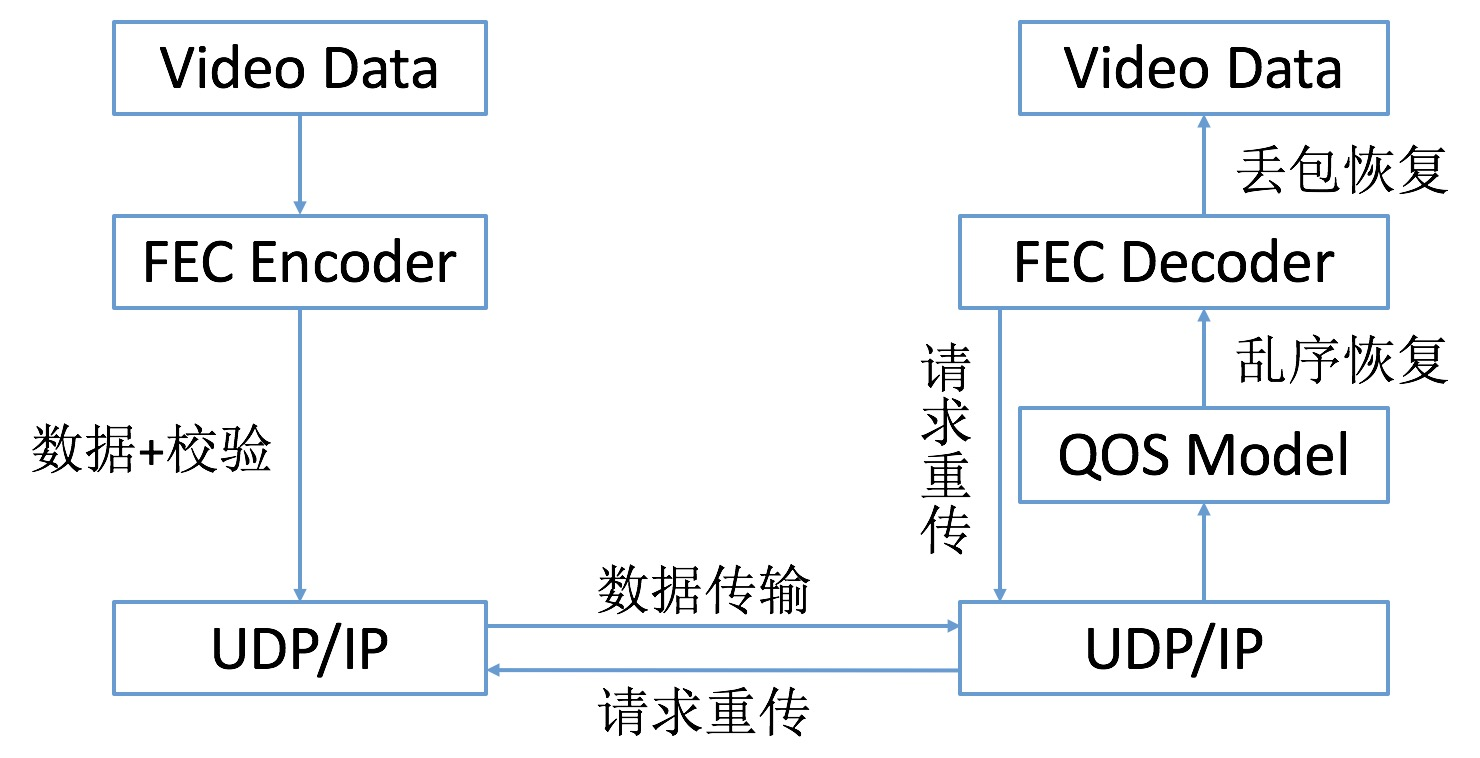
\includegraphics[width=4in]{frame.jpg}
			\caption{算法框架}
			\label{fig:frame}
		\end{figure}
		
		本算法侧重于优化具备随机信道特性的传输链路,即连续丢包的概率远低于单包丢失的情况。
		当丢包率超过前向纠错的恢复上限时,算法无法恢复所有数据,此时若要保证传输的正确性,需要引入请求重传机制。
		
		\subsection{传输协议}
		TCP和UDP是比较常用的传输协议。TCP提供可靠的通信传输,而UDP则常被用于让广播和细节控制交给应用的通信传输。
		TCP的优势在于能够提供可靠的服务,即通过TCP连接传送的数据无差错、不丢失、不重复,且按序到达,UDP不能保证可靠交付;UDP的优势在于首部开销小、占用资源少,发送数据速度更快。
		
		在本次实验中,为了追求更快的传输速度,我们采用了无连接的UDP协议,配合前向纠错和选择重传,保证传输数据的可靠性。
		
		%\subsubsection{TCP协议}
		%TCP是一种面向连接的协议,能提供可靠的传输服务,即TCP通过检验和、序列号、确认应答、重发控制、连接管理以及窗口控制等机制实现可靠性传输。TCP充分实现了数据传输时各种控制功能,可以进行丢包的重发控制,还可以对次序乱掉的分包进行顺序控制。但是这些功能也限制了TCP数据传输的速度,而且使得系统资源要求较高。
		%\subsubsection{UDP协议}
		UDP是一个非连接的协议,传输数据之前源端和终端不建立连接,当它想传送时就简单地去抓取来自应用程序的数据,并尽可能快地把它扔到网络上。在发送端,UDP传送数据的速度仅仅是受应用程序生成数据的速度、计算机的能力和传输带宽的限制;在接收端,UDP把每个消息段放在队列中,应用程序每次从队列中读一个消息段。
		
		%由于传输数据不建立连接,因此也就不需要维护连接状态,包括收发状态等,因此一台服务机可同时向多个客户机传输相同的消息。
		UDP是面向报文的。发送方的UDP对应用程序交下来的报文,在添加首部后就向下交付给IP层。既不拆分,也不合并,而是保留这些报文的边界,因此,应用程序需要选择合适的报文大小。
		
		\subsection{丢包恢复}
		
		前向纠错(FEC)技术近年来广泛应用于信息处理的各个领域。
		FEC算法通过主动提高冗余度来降低丢包重传的频率,从而降低传输延时。
		
		本次实验中的FEC算法在应用层实现,以数据包为单位进行丟包检测与丟包恢复。
		UDP协议保障了包内数据的正确性,我们无需考虑包内纠错,只处理包丢失的情况。
		每k个数据包可以生成r个冗余包,共同构成一个组(Group),即为一个独立的处理单元。
		组内每个包拥有连续的编号,通过读取编号可以判断数据包的丟失情况,并予以恢复(冗余包丢失无需恢复)。 
		
		由于冗余性的存在,一个组中任意k个包可以用来重建原始的k个数据包。
		如果丢失数据包数不超过r,即可以通过组号信息确定丟失包的相对位置并进行FEC解码,恢复k个原始媒体包。
		这里我们定义冗余包数r与原始媒体包数k的比值为FEC编码冗余度,冗余度越高,抗丟包能力越强,同时传输效率也越低。
		实际应用中,需要找到传输效率与抗丟包能力二者的折中,选择合适的冗余度配置,也可以在传输过程中动态更改。
		
		实验中采用Vandermonde矩阵RS算法,下面对算法进行简述:
		
		\subsubsection{数据包分割}
		
		对数据包进行FEC编码运算首先进行的是包内分割,将数据包分割为多个定长单元(字),实验中取字长=8bit。如图\ref{fig:FEC},FEC编码对k个原始媒体包逐字进行处理,生成r个冗余数据包中与之对应的字,包长不足的用0补齐。
		
		\begin{figure}[h]
			\centering
			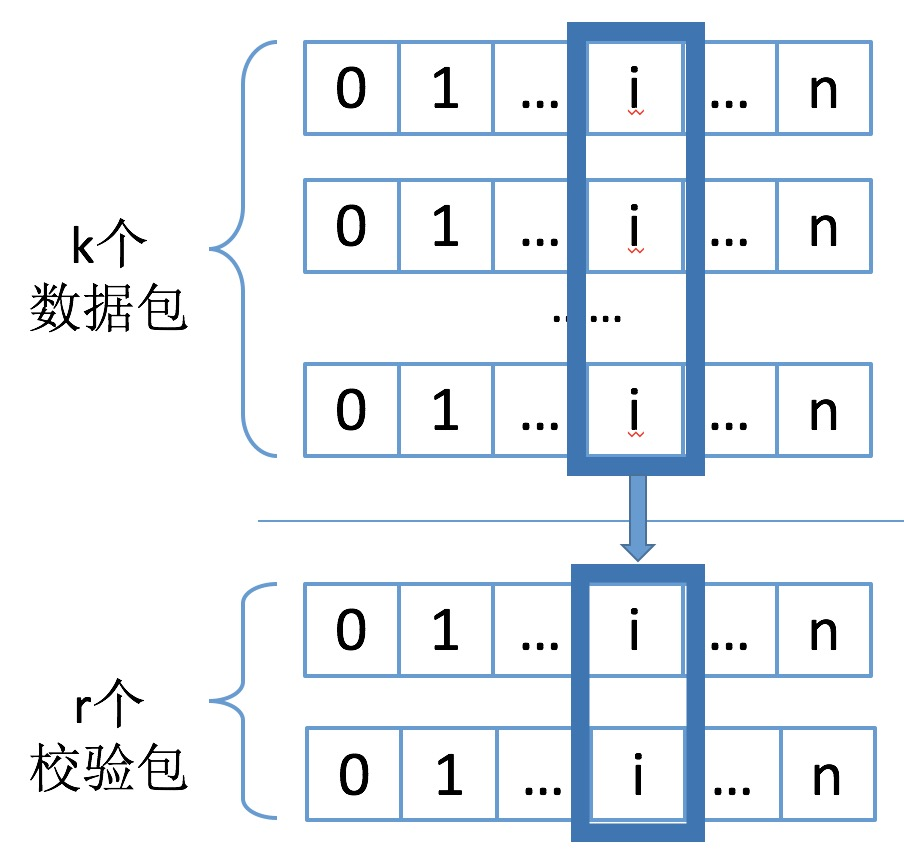
\includegraphics[width=2in]{FEC.jpg}
			\caption{前向纠错算法}
			\label{fig:FEC}
		\end{figure}
		
		\subsubsection{编解码}
		
		设k个原始数据包为$D= (D_1,D_2,\dots,D_k)$,r个冗余包为$C=(C_1,C_2,\dots,C_r)$,那么传输组可以表示为$Y= (D,C)$。
		B 为(k+r)xk维FEC生成矩阵,则组的生成满足:
		
		$$Y=BD=\left[ \begin{array}{c}I\\G\end{array} \right ]D$$
		
		在接收端,如果接收者收到了Group中的任意k个数据包,即可根据所收到的数据包在组中的位置,从FEC生成矩阵B中提取对应的行, 组成一个新的kxk维矩阵$B'$,显然
		
		$$Y'=B'D$$
		
		如果B’为非奇异矩阵,那么就可以通过如下逆变换得到原始数据包,完成恢复。
		
		$$D=(B')^{-1}Y'$$
		
		设计RS码的关键在于构造系数矩阵G。本实验中我们使用Vandermonde矩阵构建:
		
		$$G=
		\left[ \begin{array}{ccccc}
		1      & 1      & 1      & \cdots & 1       \\
		1      & 2      & 2^2    & \cdots & 2^{k-1} \\
		\vdots & \vdots & \vdots & \ddots & \vdots  \\
		1      & r      & r^2    & \cdots & r^{k-1}
		\end{array} 
		\right ]$$
		
		编解码算法中的所有元素运算都在有限域$GF(2^8)$中进行,其中加法采用位异或,乘除法通过查表计算。
		
		\subsection{乱序恢复}
		QOS模块用来处理UDP传输中的包乱序、 包重复、包延时等问题。
		
		客户端发送的每个数据包拥有递增的包序号。
		实验中使用环形队列对接收的数据包进行局部缓存并排序,同时去除接收的重复包以及超时包,最大限度保证接收质量。
		处理后的数据包按包序号从小到大输出给后面的FEC解码环节,后者进行丢包的恢复。
		
		新到数据包根据其序号和队列中已有序号进行对比,计算出其存放位置,若超出队列大小,则直接丢弃。
		设为新到包位置为$P_{new}$,$P_{out}$为即将输出的第一个数据包位置,$N_{new} $为新到包的包序号, $N_{out} $为即将输出的第一个数据包包序号,$Q_{size}$为整个环形队列大小,则:
		$$P_{new} = (P_{out} + (N_{new} - N_{out}))\%Q_{size}$$
		
		找到位置后,首先判断该位置是否已经存在数据包,如果存在,则说明当前包是重复包,直接丢弃;若不存在,则存入队列。
		
		我们用一个线程处理队列的输出,当队列中得到足以恢复一个Group的数据后,将其输出到FEC进行解码,否则保持等待。
		如果等待超过特定的丢包时延t之后,还没有得到足够的数据,就判定为数据丢失,发送丢失信号。
		
		丢包时延是算法中的一个重要参数,如果设置得过小,会发出不必要的丢失信号,系统抵御乱序的能力会变弱;如果设置得过大,则丢包重传的延时变大。
		
		\subsection{请求重传}
		本实验中的请求重传方案只对FEC确定无法恢复的数据包请求,能够尽量的降低重传发起概率,降低延时。
		
		当收到队列的丢失信号后,服务器将队列中第一个缺失数据的编号发送给客户端,由客户端的特定线程接受重传请求,立刻发出重传包。
		
\section{项目实现}
		我们使用eclipse进行android开发,使用java的socket编程实现udp协议的数据传输。
		
		\subsection{实验环境}
		\subsubsection{android客户端}
		 客户端在android手机上实现了一个应用程序。该程序具有选择文件和传输文件的功能,界面图如图\ref{fig:android}所示。\textbf{android测试环境是小米5手机,android 7.0;该应用程序要求android版本最小是andorid 6.0}。
		 
		 \begin{figure}[h]
		 	\centering
		 	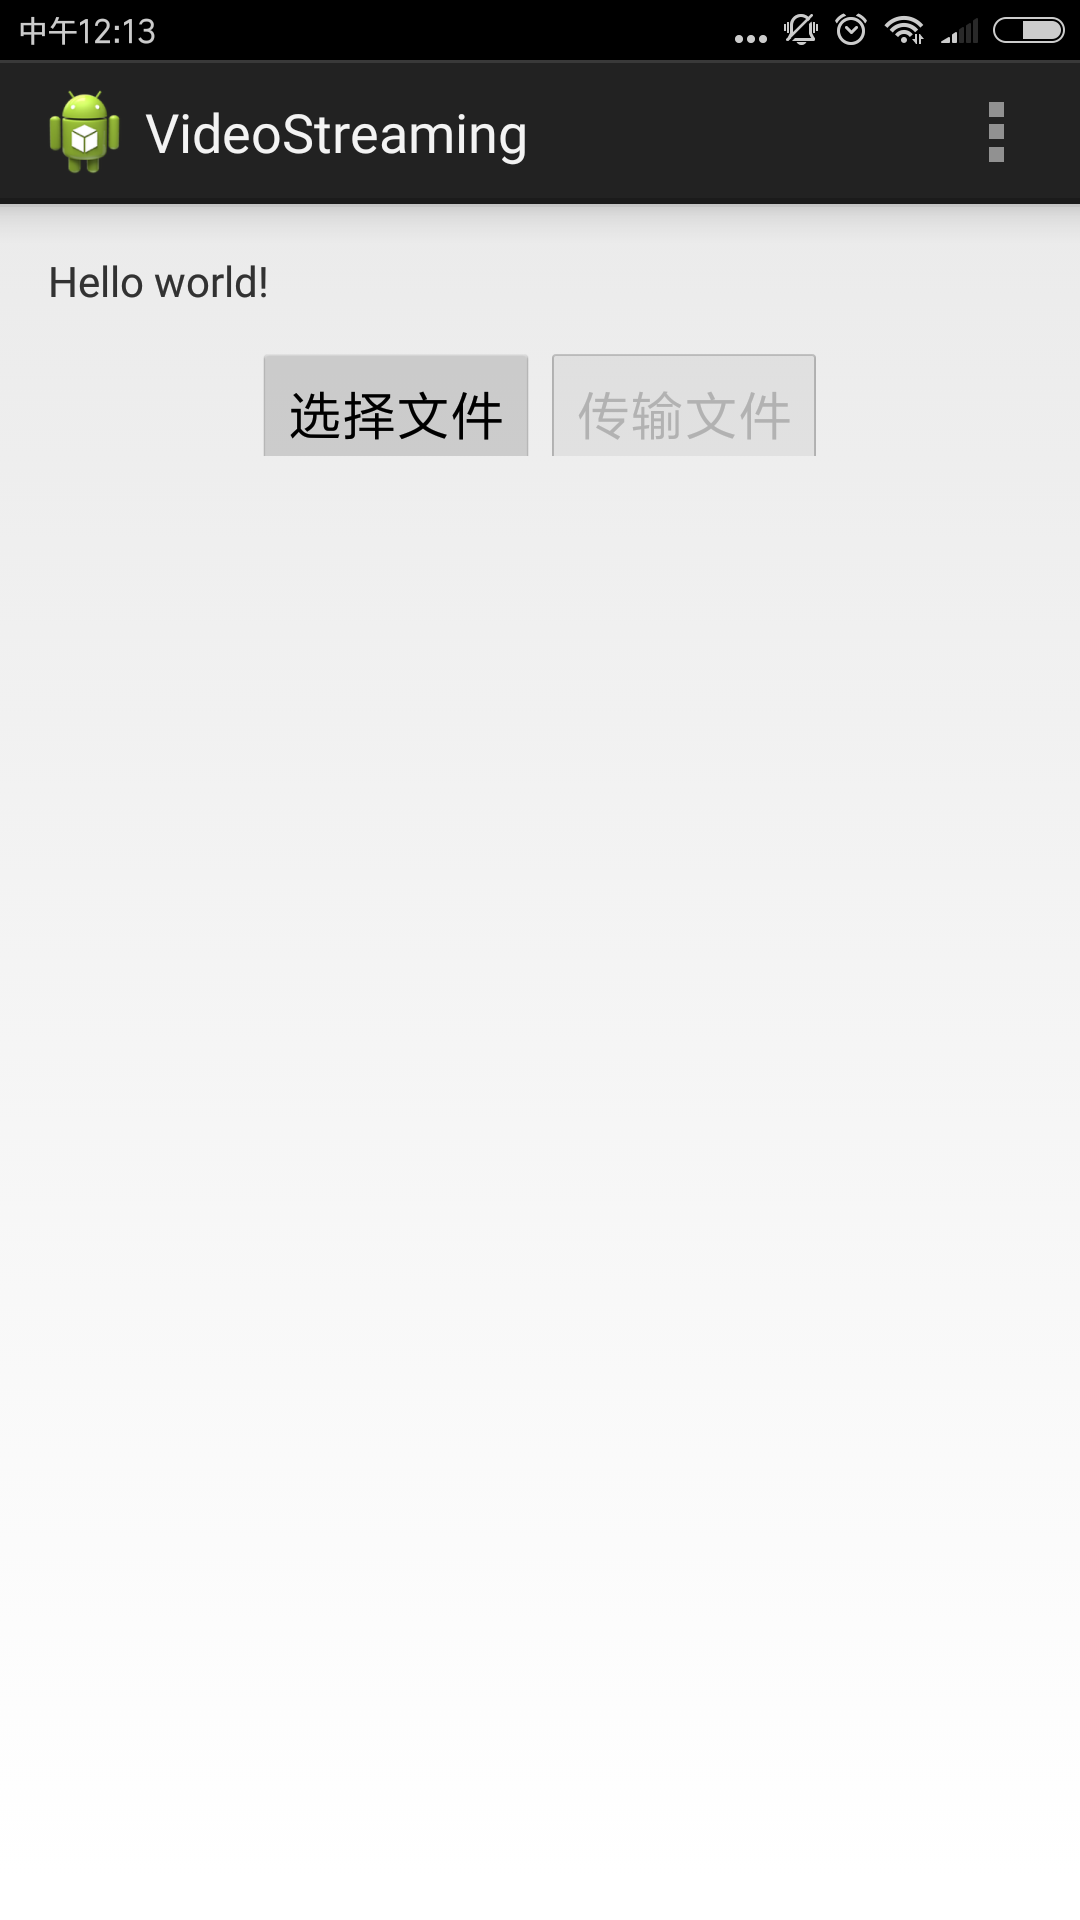
\includegraphics[width=2in]{select.png}
		 	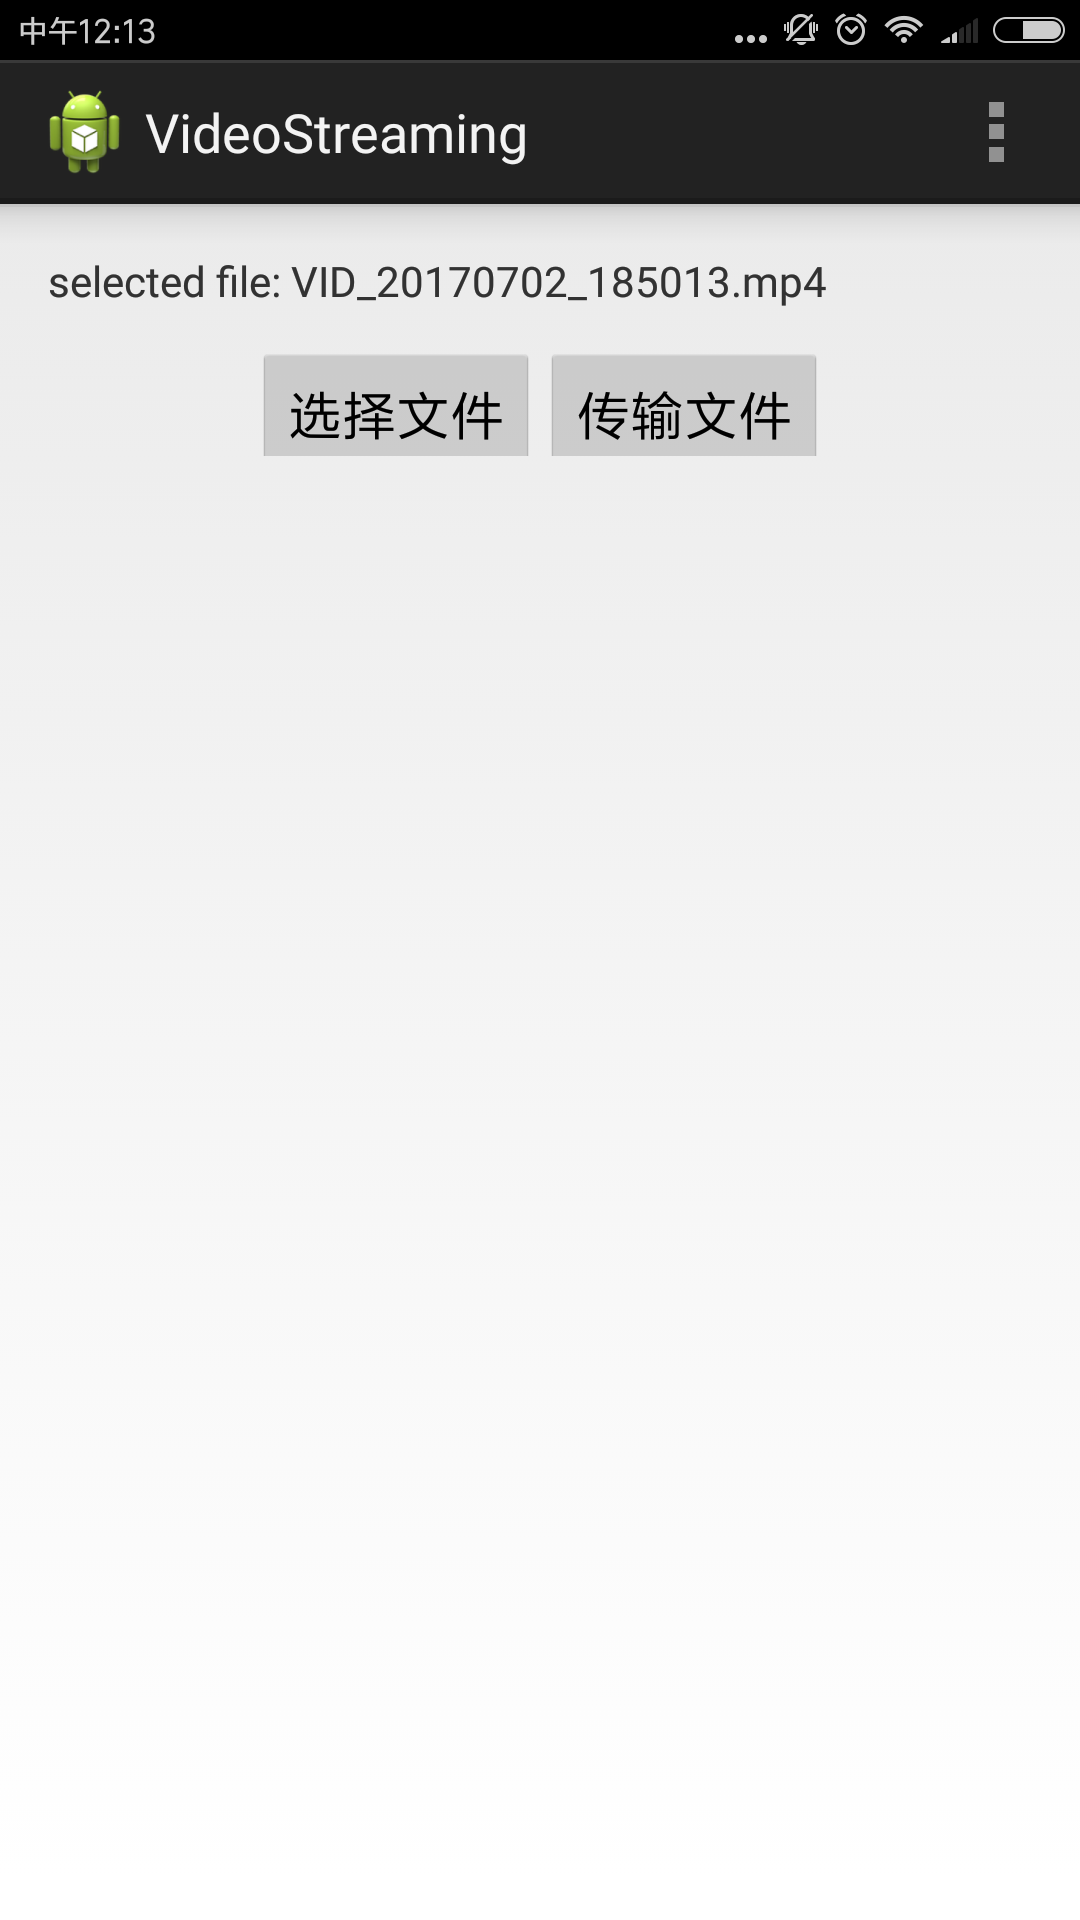
\includegraphics[width=2in]{send.png}
		 	\caption{android端程序界面}
		 	\label{fig:android}
		 \end{figure}
		 
		点击“选择文件”按钮选择想要上传的文件,选择文件后,点击“传输文件”,即开始进行文件上传。
		在点击“选择文件”按钮时,我们使用android自带的文件选择器进行文件的选择,这时会出现一个文件选择的目录,选择一个短视频,确定即回到主界面;之后我们要获得被选择文件的路径以便后续使用。在文件选择时,android6.0和以前不一样的地方在于,请求文件之前要再次申请权限,仅仅在AndroidManifest.xml文件中申请是不行的。
		
		当有文件被选择时,“传输文件”按钮被激活,点击该按钮,主程序会开启一个线程用来传输文件。该线程首先传输一个编号为0的数据包,该数据包的功能是向服务器端传输文件的信息,包括文件大小和文件名。该数据包的前两个字节表示该包的编号(一般设为0),之后四个字节表示文件大小,其他字节表示文件名。客户端发送该数据包之后会等待服务器端的特定信号(成功信号),收到该成功信号之后,客户端会继续传输文件内容;文件内容的包的前两个字节表示的是编号,该编号从1开始递增。传输文件结束,客户端会发送退出(exit)信号,在收到服务器端的成功回复后(此时服务器端也退出),客户端退出。在传输文件内容过程中,服务器端发现有丢包时,会向客户端发送重传请求,客户端收到重传请求后会暂停目前数据的传输,先重传缺失的包。
		
		\subsubsection{服务器}
		服务器端的实现是一个eclipse java程序。测试环境是windows 10 64位。在进行文件传输之前,需要先运行服务器端代码,服务器端即进行特定端口的监听,等待数据包的到来。 

		\subsection{默认参数设置}
		默认参数定义在UDPUtils.java中,包括:
		
		包大小:50KB
		
		包编号:从1开始递增
		
		FEC分组:10个数据包+2个校验包
		
		QOS环形队列大小:128
		
		请求重传时长:100ms
		
\section{实验结果与分析}
		我们采用比对文件MD5值的方式确认文件传输的正确性。实验要求首先保证传输正确,因此对无法完全恢复的组加入了请求重传。在对正确性要求没有这么高,更看中传输速度的应用中,可以取消重传模块,降低时延。
		
		\subsection{丢包率对传输速度的影响}
		保持冗余度为20\%(数据:校验=10:2),传输大小为13.52MB的视频文件,并以固定比例(不超过冗余度)随机丢包,测得丢包率和请求重传率以及传输速度之间的关系,见表\ref{table:missing_rate}。
		
		\begin{table}[h]
			\centering
		\begin{tabular}{|c|c|c|c|c|}
			\hline 
			编号 & 丢包率 & 重传率 & 传输速度(MB/s) & 正确性\\ 
			\hline 
			1 & 5\% & 3.2\% & 3.91 & 正确\\ 
			\hline 
			2 & 8\% & 5.4\% & 3.86 & 正确\\ 
			\hline 
			3 & 10\% & 6.0\% & 3.86 & 正确\\ 
			\hline 
			4 & 15\% & 8.8\% & 2.99 & 正确\\ 
			\hline 
			5 & 20\% & 9.9\% & 2.90 & 正确\\
			\hline
		\end{tabular} 
		\label{table:missing_rate}
		\end{table}
		
		对FEC算法而言,一旦组内丢包率超过冗余度,就需要请求重传。由于丢包是随机发生的,本算法不能完全恢复丢包,但能使请求重传的比例降低约50\%,从而提升传输速度。
		
		\subsection{冗余度对传输速度的影响}
		保持随机丢包率为10\%,传输大小为13.52MB的视频文件,采用不同的编码冗余度,测得冗余度和请求重传率以及传输速度之间的关系,见表\ref{table:encoding}。
		
		\begin{table}[h]
			\centering
		\begin{tabular}{|c|c|c|c|c|}
			\hline 
			编号 & 冗余度 & 重传率 & 传输速度(MB/s) & 正确性 \\ 
			\hline 
			1 & 8.3\% & 8.3\% & 3.83 & 正确 \\ 
			\hline 
			2 & 10\% & 7.4\% & 3.94 & 正确 \\ 
			\hline 
			3 & 12.5\% & 7.4\% & 4.22 & 正确 \\ 
			\hline 
			4 & 20\% & 5.8\% & 3.61 & 正确 \\ 
			\hline 
		\end{tabular} 
		\label{table:encoding}
		\end{table}
	
		可见,算法的冗余度越高,对丢失数据的恢复能力就越好,能够降低重传率,但在编解码和传输数据方面耗时更大。
		
		根据信道的丢包率选择合适的冗余度能够达到更高的传输速度,这可以通过自适应冗余度的算法实现。由于本次实验针对短视频,传输时间很短,以及代码实现方面的困难,我们没有实现自适应的功能。
		
		\subsection{请求重传中丢包时延的设置}
		保持随机丢包率为5\%,冗余度为20\%,传输大小为13.52MB的视频文件,测得请求重传中的丢包时延与重传率以及传输速度之间的关系,见表\ref{table:wait_time}。
		
		\begin{table}[h]
			\centering
			\begin{tabular}{|c|c|c|c|}
				\hline 
				编号 & 丢包时延(ms) & 重传率 & 传输速度(MB/s) \\ 
				\hline 
				1 & 80 & 4.0\% & 4.14 \\ 
				\hline 
				2 & 100 & 3.4\% & 3.52 \\ 
				\hline 
				3 & 150 & 2.5\% & 3.69 \\ 
				\hline 
			\end{tabular} 
			\label{table:wait_time}
		\end{table}
		
		可见,丢包时延越短,对乱序数据的恢复能力就越弱,但其传输速度相对更高。
		
		\subsection{总结}
		本算法可以在一定程度上恢复UDP协议带来的包丢失和包乱序问题,配合请求重传可以在保证正确性的前提下获得较高的传输速度。
		
		与短视频传输相比,本算法在对正确性要求相对较低,但对传输速度要求较高的应用场景(如直播)中,不用等待重传,并且只在丢包时引入校验的延时,能够更好的发挥其优势。
		
		
	\end{CJK*}
	
\end{document}
